\documentclass[a4paper,10pt,twocolumn]{article}
\usepackage[latin1]{inputenc}
\usepackage[english]{babel}
\usepackage{amsmath}
\usepackage{amsfonts}
\usepackage{amssymb}
\usepackage{titling}
\usepackage{nomencl}
\usepackage{booktabs}
\usepackage{graphicx}
\usepackage[style=ieee,backend=bibtex]{biblatex}
\usepackage{fancyhdr}
\usepackage{varioref}
\usepackage[activate={true,nocompatibility},final,tracking=true,kerning=true,spacing=true,factor=1100,stretch=10,shrink=10]{microtype}
% activate={true,nocompatibility} - activate protrusion and expansion
% final - enable microtype; use "draft" to disable
% tracking=true, kerning=true, spacing=true - activate these techniques
% factor=1100 - add 10% to the protrusion amount (default is 1000)
% stretch=10, shrink=10 - reduce stretchability/shrinkability (default is 20/20)

% Path to images.
\graphicspath{{img/}}

% Setup nomenclature.
\makenomenclature
\setlength{\nomitemsep}{-\parsep}

% Setup bibiliography.

% Document info.
\author{Z0966990}
\title{Statistics Assignment}
\date{\today}

% Header and footer.
\pagestyle{fancy}
\fancyhf{}
\lhead{\thetitle}
\rhead{\theauthor}
\cfoot{\thepage}
\renewcommand{\headrulewidth}{0pt}
\renewcommand{\footrulewidth}{0pt}

% Macros

\begin{document}
    
% Title page.
\begin{titlepage}
    \centering
    \vspace*{\fill}
    
\includegraphics[width=0.5\textwidth]{Durham}\\
    \vspace*{\fill}
    \LARGE\thetitle\\
    \large\theauthor\\
    \large L2 Engineering Mathematics\\
    \large\thedate\\
    \vspace*{\fill}
\end{titlepage}

% Nomenclature.
\nomenclature[0]{$n_{out}$}{Number of outliers, outside the 95\% confidence 
interval for the mean.}
\nomenclature[1]{$\bar{x}$}{Sample mean of total energy consumption.}
\printnomenclature

% Main matter.
\section{Introduction}
    
\section{Statistical Comparison}
    
\begin{figure}[h]
    \centering
    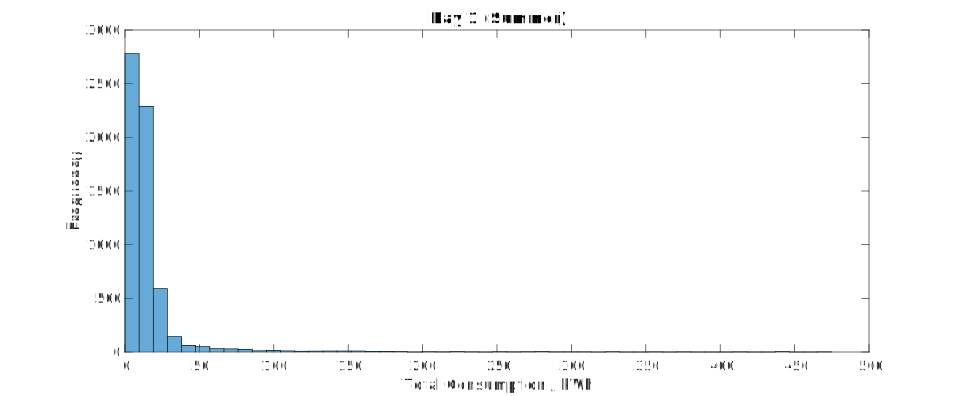
\includegraphics[width=0.42\textwidth]{Day1}
    \caption{Frequency histogram of total energy consumption on day 1.}
    \label{fig:Day1}
\end{figure}
\begin{figure}[h]
    \centering
    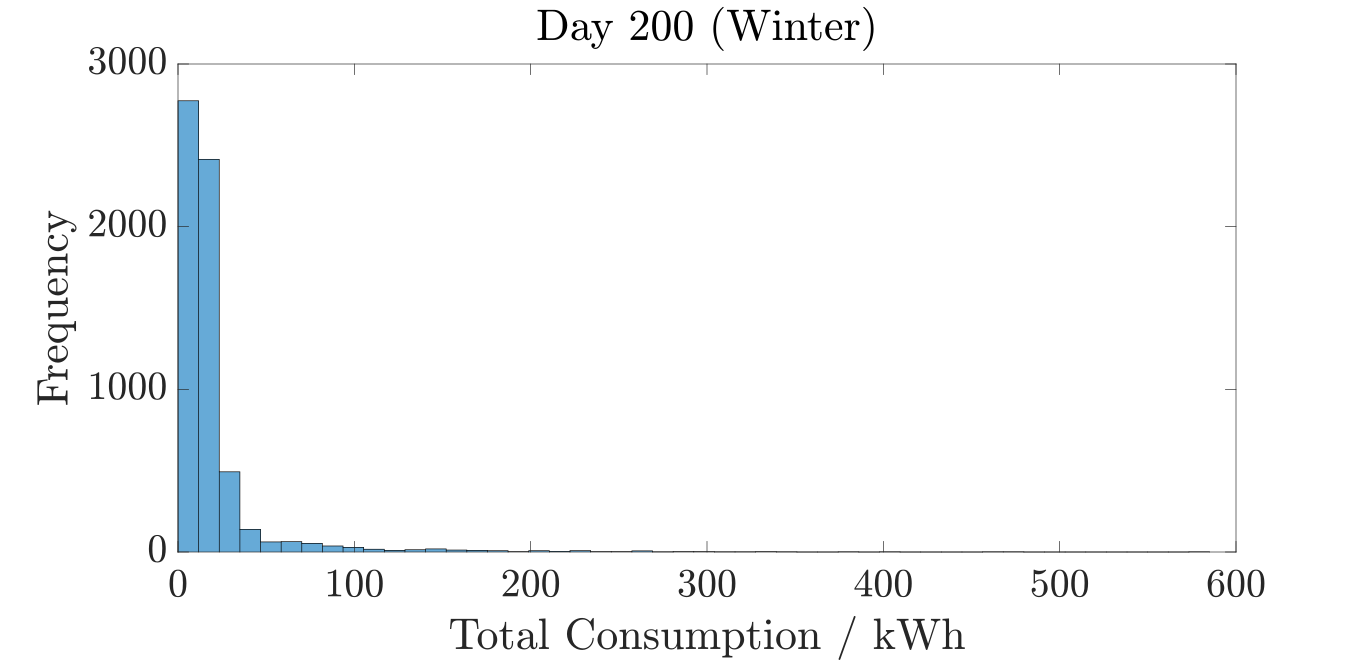
\includegraphics[width=0.42\textwidth]{Day200}
    \caption{Frequency histogram of total energy consumption on day 200.}
    \label{fig:Day200}
\end{figure}

\begin{table*}
    \centering
    \begin{tabular}{llll}
        \toprule
        \textbf{Day} & $\bar{x}$ & 90\% Interval     & 95\% Interval \\
        \midrule
        \textbf{Summer} & 30.595 & [-58.089, 119.28] & [-75.079, 136.27] \\
        \textbf{Winter} & 39.265 & [-64.566, 143.10] & [-84.457, 162.99] \\
        \bottomrule
    \end{tabular}
    \caption{Confidence intervals for mean energy consumption on each day.}
    \label{table:Mean}
\end{table*}

\section{Outlier Analysis}


\begin{figure}[h]
    \centering
    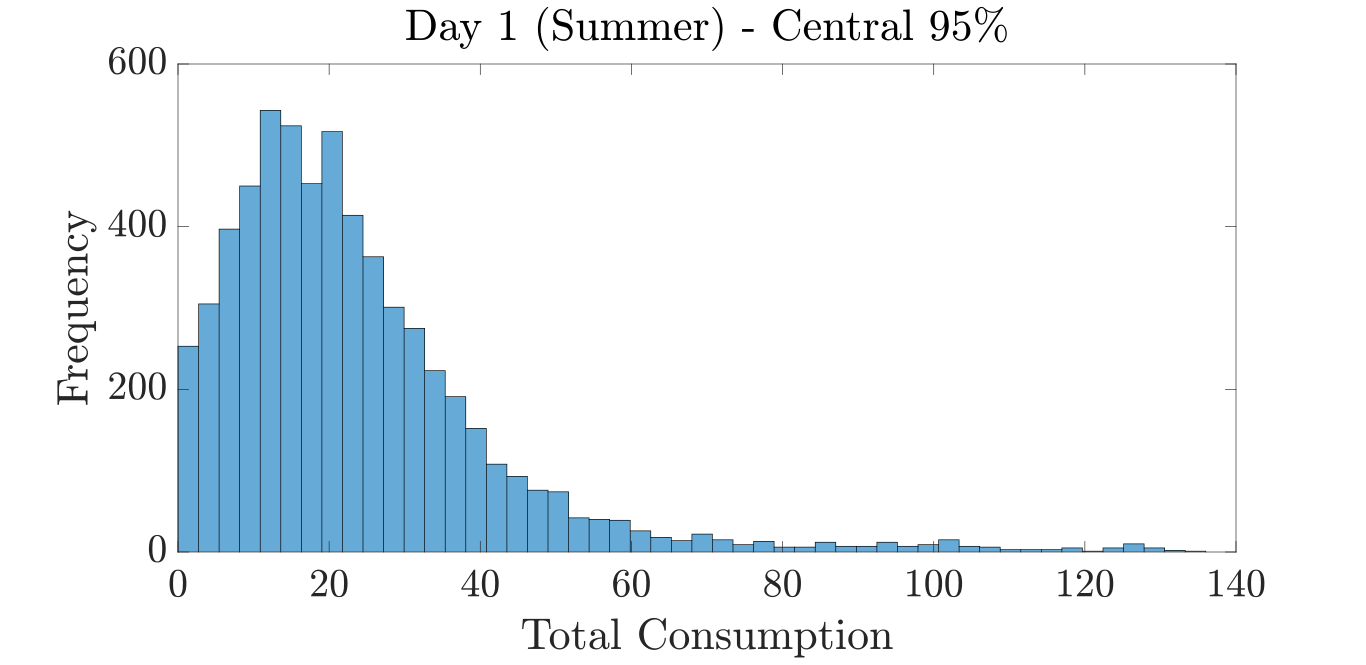
\includegraphics[width=0.42\textwidth]{Day1Central95}
    \caption{Frequency histogram of central 95\% of total energy consumption on 
    day 1.}
    \label{fig:NoOutliers}
\end{figure}

\begin{table}
    \centering
    \begin{tabular}{llll}
        \toprule
        \textbf{Sample \%} & $\bar{x}$ & 95\% Interval & 
        $n_{out}$ \\
        \midrule
        \textbf{100\%} & 30.595 & [-75.079, 136.27] & 174 \\
        \textbf{95\%}  & 39.265 & [-12.887, 59.708] & 250 \\
        \bottomrule
    \end{tabular}
    \caption{Number of outliers for the central 100\% and 95\% of total energy 
    consumption on day 1.}
    \label{table:Outliers}
\end{table}

% References.
\printbibliography

\clearpage

\end{document}